\documentclass[11pt,a4paper]{article}
\usepackage[margin=24mm]{geometry}
\usepackage{fontspec}
\setmainfont{TeX Gyre Termes}
\setmonofont[Scale=0.86]{Latin Modern Mono}
\usepackage{amsmath,amssymb,graphicx,booktabs,longtable,tabularx}
\usepackage[font=small,labelfont=bf]{caption}
\usepackage{xcolor,hyperref,fancyhdr}
\hypersetup{colorlinks=true,linkcolor=blue!40!black,urlcolor=blue!40!black,
pdftitle={TRACE-Q: Supplementary Material}}
\pagestyle{fancy}\fancyhf{}
\fancyhead[L]{\small TRACE-Q: Supplementary material}\fancyfoot[C]{S\thepage}
\setlength{\headheight}{14pt}
\setlength{\parskip}{3pt}\setlength{\emergencystretch}{2em}
\renewcommand{\thetable}{S\arabic{table}}
\renewcommand{\thefigure}{S\arabic{figure}}
\begin{document}
\begin{center}{\Large\bfseries TRACE-Q: Supplementary Material}\end{center}

\section{Paper-Level Results}
\small
\begin{longtable}{llrrrrr}
\caption{Per-paper counts derived from the final human workbooks.}\label{tab:perpaper}\\
\toprule
Year & Paper DOI suffix & Candidates & Retained & Primary & Strict & Secondary \\
\midrule
\endfirsthead
\toprule
Year & Paper DOI suffix & Candidates & Retained & Primary & Strict & Secondary \\
\midrule
\endhead
\bottomrule
\endfoot
2018 & \texttt{jama.2017.21906} & 7 & 6 & 1 & 0 & 0 \\
2018 & \texttt{jama.2018.0156} & 8 & 7 & 1 & 1 & 0 \\
2018 & \texttt{jama.2018.0948} & 12 & 11 & 0 & 0 & 0 \\
2018 & \texttt{jama.2018.14280} & 10 & 10 & 1 & 1 & 0 \\
2018 & \texttt{jama.2018.14282} & 16 & 16 & 3 & 3 & 1 \\
2018 & \texttt{jama.2018.17075} & 15 & 15 & 2 & 1 & 0 \\
2018 & \texttt{jama.2018.18020} & 22 & 21 & 5 & 4 & 0 \\
2018 & \texttt{jama.2018.6496} & 13 & 11 & 0 & 0 & 0 \\
2018 & \texttt{jama.2018.8802} & 5 & 4 & 1 & 1 & 0 \\
2018 & \texttt{jama.2018.9128} & 7 & 6 & 0 & 0 & 0 \\
2019 & \texttt{jama.2019.0556} & 11 & 11 & 1 & 0 & 0 \\
2019 & \texttt{jama.2019.10517} & 5 & 5 & 0 & 0 & 0 \\
2019 & \texttt{jama.2019.12618} & 10 & 10 & 0 & 0 & 0 \\
2019 & \texttt{jama.2019.14630} & 9 & 9 & 1 & 1 & 0 \\
2019 & \texttt{jama.2019.14901} & 5 & 5 & 0 & 0 & 0 \\
2019 & \texttt{jama.2019.17380} & 18 & 18 & 0 & 0 & 0 \\
2019 & \texttt{jama.2019.2210} & 7 & 5 & 0 & 0 & 0 \\
2019 & \texttt{jama.2019.4755} & 1 & 1 & 0 & 0 & 0 \\
2019 & \texttt{jama.2019.7505} & 13 & 12 & 4 & 4 & 0 \\
2024 & \texttt{jama.2024.0318} & 14 & 14 & 0 & 0 & 0 \\
2024 & \texttt{jama.2024.0572} & 19 & 16 & 5 & 5 & 0 \\
2024 & \texttt{jama.2024.11057} & 5 & 5 & 0 & 0 & 0 \\
2024 & \texttt{jama.2024.12829} & 7 & 7 & 1 & 1 & 0 \\
2024 & \texttt{jama.2024.19585} & 7 & 5 & 0 & 0 & 0 \\
2024 & \texttt{jama.2024.2302} & 6 & 6 & 1 & 1 & 0 \\
2024 & \texttt{jama.2024.23898} & 13 & 13 & 0 & 0 & 0 \\
2024 & \texttt{jama.2024.25786} & 15 & 14 & 1 & 1 & 0 \\
2024 & \texttt{jama.2024.4183} & 14 & 14 & 1 & 1 & 0 \\
2024 & \texttt{jama.2024.6063} & 13 & 13 & 2 & 2 & 0 \\
2025 & \texttt{jama.2024.24764} & 5 & 5 & 1 & 1 & 0 \\
2025 & \texttt{jama.2024.27643} & 16 & 13 & 2 & 2 & 1 \\
2025 & \texttt{jama.2025.11178} & 18 & 17 & 3 & 3 & 0 \\
2025 & \texttt{jama.2025.15185} & 6 & 6 & 1 & 1 & 0 \\
2025 & \texttt{jama.2025.15440} & 1 & 1 & 0 & 0 & 0 \\
2025 & \texttt{jama.2025.16450} & 6 & 5 & 0 & 0 & 0 \\
2025 & \texttt{jama.2025.19563} & 13 & 10 & 0 & 0 & 0 \\
2025 & \texttt{jama.2025.19843} & 7 & 7 & 0 & 0 & 0 \\
2025 & \texttt{jama.2025.20765} & 19 & 19 & 1 & 1 & 1 \\
2025 & \texttt{jama.2025.24175} & 14 & 14 & 2 & 2 & 1 \\
2025 & \texttt{jama.2025.4390} & 13 & 13 & 0 & 0 & 0 \\
2025 & \texttt{jama.2025.7583} & 4 & 4 & 0 & 0 & 0 \\
2025 & \texttt{jama.2025.7710} & 3 & 3 & 0 & 0 & 0 \\
2025 & \texttt{jama.2025.9110} & 3 & 2 & 0 & 0 & 0 \\
2025 & \texttt{jama.2025.9663} & 5 & 4 & 0 & 0 & 0 \\
\end{longtable}
\normalsize
\noindent\footnotesize DOI prefix is 10.1001/. Primary = substantive confirmed/probable statistical issues; strict = substantive confirmed statistical issues; secondary = substantive report-internal inconsistencies. All three require an original report-only relationship.\normalsize


\section{Adjudication and Analysis Details}
The analysis reads the four completed Excel workbooks directly, using stable candidate keys to join original relationship codes. It checks unique keys, row totals, completion, and required domain-specific judgments. All 440 supplied human decisions are preserved. Final human domains determine descriptive summaries; original document relationships additionally constrain temporal eligibility. Candidate \texttt{2024::jama.2024.11057::C003}, for example, was retained as a substantive report-internal inconsistency after domain editing, but its original \texttt{P\_R} relationship excludes it from the secondary temporal endpoint. It remains in the descriptive human-domain total.

The 149 confirmed report-material issues of any substantiveness occurred in 38 of 44 papers. This broader count includes minor presentation issues and differs from the principal endpoint of 41 confirmed or probable substantive statistical issues. The broad count is descriptive and is not a detection-accuracy measure.

\subsection{Illustrative Human Decisions}
For \texttt{jama.2018.14280}, C001 concerned the identity of a reported binary risk ratio and was retained as a confirmed substantive statistical issue with direct potential impact on extraction. For \texttt{jama.2017.21906}, C001 compared a planned medication composite containing statin use with the reported composite; the report disclosed that statin data were not collected. This was retained as a substantive protocol--report difference without an inference of unjustified change. For \texttt{jama.2018.0156}, C002 was excluded because secondary-outcome and safety-analysis descriptions could coexist within the supplied plans. These examples summarize final adjudications, rather than proposing corrected results.

\begin{table}[tbp]
\centering\small
\caption{Candidate dispositions using the final human review domains.}
\label{tab:dispositions}
\begin{tabular}{lrrrr}
\toprule
Review domain & Candidates & Retained & Excluded & Retained (\%) \\
\midrule
Statistical results & 173 & 155 & 18 & 89.6 \\
Report internal inconsistency & 12 & 12 & 0 & 100.0 \\
Protocol--report & 216 & 214 & 2 & 99.1 \\
Planning material & 39 & 32 & 7 & 82.1 \\
\bottomrule
\end{tabular}
\par\vspace{4pt}\begin{minipage}{0.97\linewidth}\footnotesize Five candidates changed domain during human review. Protocol--report differences and planning-material findings are descriptive; they do not enter the temporal endpoints.\end{minipage}
\end{table}


\subsection{Full Period Comparisons}
Table~\ref{tab:temporal} gives the complete set of exploratory comparisons, including binary sensitivity endpoints omitted from the main table for space. All tests reallocate papers between groups of 19 and 25; candidates remain grouped within their papers. Exact probabilities count all allocations with a statistic at least as extreme in absolute value, including ties. Bootstrap intervals resample papers within periods and are not permutation intervals.
\begin{table}[tbp]
\centering\small
\caption{Exploratory comparison of report-material outcomes between publication periods.}
\label{tab:temporal}
\begin{tabular}{>{\raggedright\arraybackslash}p{5.0cm}rrrr}
\toprule
Outcome & 2018--2019 & 2024--2025 & Difference (95\% CI) & $P$ \\
\midrule
Substantive statistical (count) & 1.05 & 0.84 & -0.21 (-1.02, 0.56) & 0.654 \\
Substantive statistical (any) & 10/19 & 12/25 & -4.6 (-33.7, 25.7) & 1.000 \\
Substantive report inconsistency (count) & 0.05 & 0.12 & 0.07 (-0.09, 0.24) & 0.622 \\
Substantive report inconsistency (any) & 1/19 & 3/25 & 6.7 (-9.1, 24.0) & 0.622 \\
Confirmed statistical only (count) & 0.84 & 0.84 & 0.00 (-0.77, 0.74) & 1.000 \\
Confirmed statistical only (any) & 8/19 & 12/25 & 5.9 (-24.4, 35.2) & 0.766 \\
Combined substantive report (count) & 1.11 & 0.96 & -0.15 (-1.02, 0.68) & 0.754 \\
Combined substantive report (any) & 10/19 & 12/25 & -4.6 (-33.7, 25.7) & 1.000 \\
\bottomrule
\end{tabular}
\par\vspace{4pt}\begin{minipage}{0.97\linewidth}\footnotesize Count rows show the mean number per paper; any rows show papers with at least one eligible issue. Differences are later minus earlier, in issues per paper or percentage points, respectively. Principal-endpoint eligibility includes confirmed or probable statistical issues judged substantive. The confirmed-only and combined endpoints are sensitivity analyses. Confidence intervals use 20,000 paper bootstrap resamples within periods; two-sided permutation $P$ values are exact and unadjusted. No protocol--report or planning-material finding contributes.\end{minipage}
\end{table}


\begin{figure}[tbp]
\centering
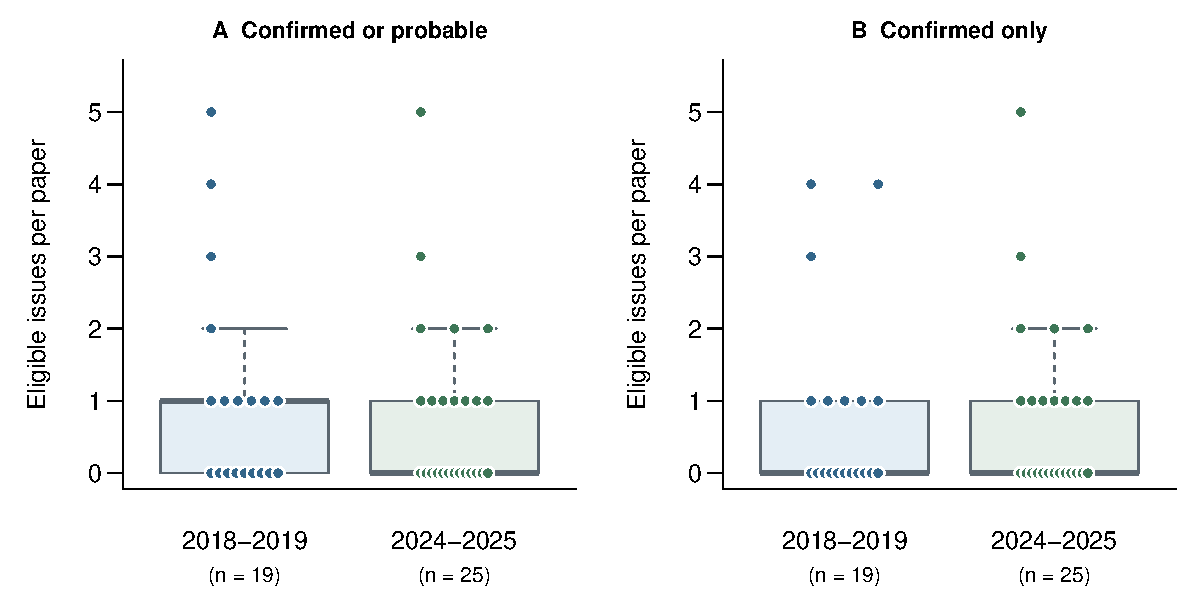
\includegraphics[width=\linewidth]{figures/period_counts.pdf}
\caption{Substantive statistical issues by publication period. Each point represents a paper, including zero counts. Panel A includes confirmed and probable issues; Panel B includes confirmed issues only. Boxes show medians and interquartile ranges; whiskers extend to observations within 1.5 interquartile ranges.}
\label{fig:period}
\end{figure}

\subsection{Interpretation of Review Fields}
\begin{table}[htbp]
\centering\small
\caption{Operational interpretation of final human review fields.}
\label{tab:codebook}
\begin{tabularx}{\linewidth}{p{3.5cm}X}
\toprule
Field & Interpretation used in the analysis \\
\midrule
Disposition & Retain, exclude, or discuss; blank means unanswered. Retention alone is not confirmation. \\
Statistical issue & Confirmed, probable, not an issue, or indeterminate; required for retained statistical candidates. \\
Substantiveness & Substantive, minor presentation, or indeterminate; separate from evidential certainty. \\
Downstream impact & Optional direct, possible, unlikely, or unknown impact; not an eligibility criterion or evidence of actual harm. \\
Internal inconsistency & Substantive, minor presentation, no inconsistency, or indeterminate; used for report-internal and planning-material candidates. \\
Protocol interpretation & Optional description of a difference or ambiguity; excluded from temporal endpoints regardless of apparent importance. \\
Completion & \texttt{primary\_done} indicates a completed review entry, not scientific confirmation. \\
\bottomrule
\end{tabularx}
\end{table}

\section{Reproducible Computation}
The files \path{candidate_results.csv} and \path{paper_results.csv} preserve analysis variables. The file \path{period_comparisons.csv} contains unrounded estimates, intervals, and exact permutation probabilities. Original candidate domain and relationship codes are stored separately from final human labels. The R script cross-checks its dynamic-programming calculation against direct enumeration of a small example with tied and zero counts; an independent implementation reproduced all eight reported permutation probabilities. All 44 papers enter the analysis, including those with no eligible finding. The manuscript tables use final workbooks rather than historical preliminary counts in project correspondence.

The source archive contains 188 PDFs (5,559 pages) and one Excel worksheet. Thus, 5,560 is the number of mixed source units, not the number of PDF pages. Source-file and report hashes are retained with the analysis. The project notes document the initial feasibility exercise and the rationale for separating broad descriptive review from narrower temporal outcomes; the main paper does not treat these notes as published evidence or the pilot as independent validation.
\end{document}
